\documentclass[conference]{IEEEtran}
\IEEEoverridecommandlockouts
\usepackage{cite}
\usepackage{amsmath,amssymb,amsfonts}
\usepackage{graphicx}
\usepackage{booktabs}
\usepackage{multirow}
\usepackage{xcolor}
\usepackage{xurl}
\usepackage{tikz}
\usetikzlibrary{arrows.meta,positioning}
% Draft markers: red text must be checked or filled before submission.
\newcommand{\todo}[1]{\textcolor{red}{[TODO: #1]}}

\begin{document}

\title{Pattern-Aware Spectrum Reservation and Grouped\\Push-Pull Defragmentation in Elastic Optical Networks}

\author{\IEEEauthorblockN{Mohammad Mahdi Malayeri}
\IEEEauthorblockA{\textit{Dept. of Computer Engineering and IT}\\
\textit{University of Qom}\\
Qom, Iran \\
malayerimahdi@gmail.com}
\and
\IEEEauthorblockN{Mohsen Nickray}
\IEEEauthorblockA{\textit{Dept. of Computer Engineering and IT}\\
\textit{University of Qom}\\
Qom, Iran \\
\todo{email}}
% TODO: confirm both affiliations
}

\maketitle

\begin{abstract}
Spectrum fragmentation causes connection requests in elastic optical networks (EONs) to be blocked even when enough total capacity is free. This paper asks whether recognizing recurring traffic patterns can reduce this blocking. We detect periodic flows from the request stream and use them in three ways: advance spectrum reservation, a separate spectrum zone for periodic flows, and holding spectrum between repeats. These are combined with non-disruptive Push-Pull defragmentation, whose shift operations are grouped into parallel rounds with a greedy maximal-independent-set algorithm. Simulations on the 14-node NSFNET topology with 10 independent runs per point show that Push-Pull reduces bandwidth blocking by 31--92\% compared with First-Fit, and route grouping cuts the number of sequential shift operations by 2.5--3.3$\times$. Periodic flows are detected with a precision of 1.00 and a recall of 0.86--0.92. No use of the detected patterns lowers total blocking: holding spectrum lowers the blocking of periodic flows by 25--36\% at 80--120 Erlang and the zone policy cuts defragmentation moves by 42--60\%, but both raise the blocking of other traffic. The trade-off can be tuned. Reserving spectrum about one tenth of a period ahead protects periodic flows by 29--44\% with no significant change in total blocking, a better trade-off than holding. A detection tolerance of three times the timing jitter keeps the recall above 0.8. Pattern awareness therefore does not create capacity; it decides which traffic receives it, which is useful for protecting scheduled services.
\end{abstract}

\begin{IEEEkeywords}
elastic optical networks, spectrum fragmentation, Push-Pull defragmentation, traffic patterns, spectrum reservation, independent sets
\end{IEEEkeywords}

% ===============================================================
\section{Introduction}
% ===============================================================
Elastic optical networks (EONs) divide the optical spectrum into fine-grained frequency slots (FSs) and allocate to each connection only as many contiguous slots as it needs \cite{jinno2009,gerstel2012}. A lightpath must occupy the same contiguous block of slots on every link of its route \cite{chatterjee2015}. As connections with different bandwidths and holding times are set up and released, the free spectrum breaks into small, non-aligned gaps, and a new request can be blocked even though enough total capacity is free. This spectrum fragmentation is one of the main obstacles to the efficient operation of dynamic EONs.

Fragmentation-aware routing and spectrum assignment (RSA) tries to avoid creating unusable gaps \cite{shen2015,abkenar2017}, while defragmentation re-arranges active connections to consolidate free spectrum \cite{patel2011,wang2013,zhang2013,cugini2013}. Both act on the current spectrum state. Real traffic, however, is not purely random: scheduled services such as IPTV and video on demand repeat between the same node pairs with nearly constant intervals and bandwidths. A natural idea is to recognize such patterns and act before the requests arrive, an approach explored in the MSc thesis on which this paper builds \cite{malayeri2022}.

This paper tests that idea carefully. Its contributions are:
\begin{itemize}
\item A periodic-flow detector that runs on the request stream, and three ways to use its output: advance reservation, a separate spectrum zone, and holding spectrum between repeats.
\item A grouped Push-Pull defragmentation in which routes that share no link are shifted in parallel, using a greedy maximal-independent-set partition \cite{shakya2013}.
\item An evaluation on NSFNET with 10 seeds per point and 95\% confidence intervals, which shows clearly what pattern awareness can and cannot achieve: it redistributes spectrum between traffic classes but does not lower total blocking.
\item A study of the knobs that tune this redistribution, namely the reservation lead time, a budget on held spectrum, and the detection tolerance under timing jitter, which identifies advance reservation with a moderate lead as the most efficient way to protect periodic flows.
\item An open-source simulator with all experiments and results.\footnote{\url{https://github.com/malayerimahdi/EON-Pattern-Aware-Spectrum-Management}}
\end{itemize}

Section~\ref{sec:related} reviews related work, Section~\ref{sec:model} defines the model, Section~\ref{sec:method} describes the methods, Section~\ref{sec:setup} the setup, Section~\ref{sec:results} the results, and Section~\ref{sec:conclusion} concludes the paper.

% ===============================================================
\section{Related Work}\label{sec:related}
% ===============================================================
\textit{RSA and defragmentation.} Surveys of RSA in EONs are given in \cite{chatterjee2015,abkenar2017}. Fragmentation-aware RSA chooses spectrum positions that limit small gaps \cite{shen2015,athari2019}. Defragmentation re-arranges active lightpaths \cite{patel2011}; make-before-break and non-disruptive variants limit service interruption \cite{wang2013,zhang2013}. Push-Pull shifts a lightpath to adjacent free spectrum without disrupting its traffic \cite{cugini2013}, and independent sets of routes allow several lightpaths to be defragmented in parallel \cite{shakya2013}.

\textit{Traffic-aware allocation.} Advance reservation, where requests are known before they start, allows better planning of spectrum use \cite{lu2013ar}. Spectrum allocation adapted to estimated traffic fluctuations was studied in \cite{chino2016}, and machine learning has been applied to bandwidth allocation \cite{panayiotou2019} and quality-of-transmission-aware RSA \cite{salani2019}. Learning has recently been applied to defragmentation itself: deep reinforcement learning selects which connections to re-allocate and when \cite{etezadi2022,etezadi2023}, a classifier triggers defragmentation when the predicted blocking rate exceeds a threshold \cite{davalos2023}, and cognitive control loops diagnose and act on degraded network states \cite{trindade2021}. These works learn \emph{when} or \emph{how} to defragment. We instead learn \emph{which demands recur} from the request stream itself, and we measure, under identical traffic, how each way of using this knowledge affects blocking and defragmentation cost.

% ===============================================================
\section{Network and Traffic Model}\label{sec:model}
% ===============================================================
The network is a graph $G=(V,E)$ in which each link carries $S$ frequency slots. A request is $r=(t_r, s_r, d_r, b_r, h_r)$: arrival time, source, destination, number of FSs, and holding time. It is served on one of the $k$ shortest paths between $s_r$ and $d_r$ if $b_r$ plus a guard band of contiguous FSs are free on every link at the same position; otherwise it is blocked.

Traffic follows the OPNET generator of \cite{malayeri2022}: Poisson arrivals, uniformly chosen node pairs, $b_r$ uniform in 5--20 FSs, and exponential holding times with mean $\bar{h}=20$. On top of this random traffic, $F$ periodic flows each repeat a fixed $(s,d,b)$ with a constant period. A share $\phi$ of the offered load $A$ (in Erlang) comes from the periodic flows; random requests arrive at rate $(1-\phi)A/\bar{h}$, and each periodic flow has period $T = F\bar{h}/(\phi A)$.

% ===============================================================
\section{Methods}\label{sec:method}
% ===============================================================
Fig.~\ref{fig:pipeline} shows how the components fit together.

\begin{figure}[t]
\centering
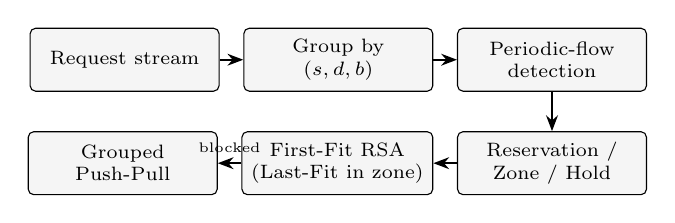
\begin{tikzpicture}[
  box/.style={draw, rounded corners=2pt, align=center, font=\scriptsize, minimum width=2.4cm, minimum height=0.8cm, fill=gray!8},
  arr/.style={-{Stealth[length=2mm]}, thick}]
\node[box] (a) {Request stream};
\node[box, right=0.3cm of a] (b) {Group by\\$(s,d,b)$};
\node[box, right=0.3cm of b] (c) {Periodic-flow\\detection};
\node[box, below=0.5cm of c] (d) {Reservation /\\Zone / Hold};
\node[box, left=0.3cm of d] (e) {First-Fit RSA\\(Last-Fit in zone)};
\node[box, left=0.3cm of e] (f) {Grouped\\Push-Pull};
\draw[arr] (a)--(b); \draw[arr] (b)--(c); \draw[arr] (c)--(d); \draw[arr] (d)--(e);
\draw[arr] (e)--node[above, font=\tiny]{blocked} (f);
\end{tikzpicture}
\caption{Components of the pattern-aware scheme.}
\label{fig:pipeline}
\end{figure}

\subsection{Grouped Push-Pull Defragmentation}
When a request is blocked, Push-Pull \cite{cugini2013} shifts every active lightpath, in order of its lowest slot, to the lowest position it can reach through contiguous free slots. A shift never jumps over another lightpath, so it does not disrupt traffic. The request is then tried again. Shifts on routes that share no link can run in parallel. We build a conflict graph of the moved routes and repeatedly remove a maximal independent set, choosing shorter routes first \cite{shakya2013}; each set is one parallel round. The number of rounds, rather than the number of shifts, sets the defragmentation time.

\subsection{Periodic-Flow Detection}
Requests are grouped by key $(s,d,b)$. For the last four arrivals $t_1<\dots<t_4$ of a key, the key is marked periodic with period $T$ if
\begin{equation}
\left| (t_{i+1}-t_i) - T \right| \le \varepsilon,\quad i=1,2,3,
\end{equation}
where $T$ is the mean interval and $\varepsilon=0.1$. A key loses its mark as soon as an interval breaks the pattern. This rule generalizes the stream-based pattern finder of the thesis \cite{malayeri2022}.

\subsection{Three Uses of Detected Patterns}
\textit{Reservation.} A time $\delta=0.2$ before the next expected arrival of a periodic key, a block of $b$ FSs is reserved on its route (with Push-Pull if needed). The arriving request takes the block; if it does not arrive within $\varepsilon+\delta$ of the expected time, the block is released.

\textit{Zone.} Detected periodic flows are placed with Last-Fit, at the top of the band, while other traffic uses First-Fit from the bottom; Push-Pull pushes periodic connections up and others down. The goal is to keep the two classes from fragmenting each other.

\textit{Hold.} When a connection of a periodic key ends and its next repeat is still expected, its block is kept for that repeat instead of being released.

\textit{Hold with a budget.} Held blocks sit idle until the next repeat. To control how much spectrum this costs, a block is held only if, on every link of its route, the slots already idle in held or reserved blocks plus the new block stay within a share $\beta$ of the $S$ slots; otherwise it is released as usual. $\beta=1$ is unrestricted Hold and $\beta\to 0$ is FF+PP.

\subsection{Complexity}
Detection keeps the last four arrival times per key and costs $O(1)$ per request. A First-Fit search on a path of $\ell$ links costs $O(\ell S)$. One Push-Pull pass over $n$ active lightpaths costs $O(n\,\ell S)$ in the worst case, and the greedy grouping of $m$ moved routes costs $O(m^2\ell)$, which is negligible next to the shift operations it schedules.

\subsection{Per-Pair Demand Prediction}
We also test whether demand can be predicted per node pair, as proposed in \cite{malayeri2022}. Time is divided into windows; for each pair, a decision tree (depth 5) predicts from the demands of the previous three windows whether the next window's demand will exceed the transmission threshold, defined as the mean demand per pair and window. The first 70\% of windows are used for training and the rest for testing.

% ===============================================================
\section{Simulation Setup}\label{sec:setup}
% ===============================================================
We use a Python discrete-event simulator on the 14-node, 21-link NSFNET topology with real link lengths (300--2800\,km). Table~\ref{tab:params} lists the parameters. After every run, a consistency check verifies that the spectrum map matches the active connections and that no lightpaths overlap.

\begin{table}[t]
\centering
\caption{Simulation parameters}
\label{tab:params}
\small
\begin{tabular}{@{}ll@{}}
\toprule
Parameter & Value \\
\midrule
FSs per link $S$ / guard band & 320 / 1 FS \\
Routing / assignment & 3 shortest paths / First-Fit \\
Demand $b_r$ & uniform, 5--20 FSs \\
Mean holding time $\bar{h}$ & 20 \\
Periodic flows $F$ / share $\phi$ & 20 / 0.3 (unless stated) \\
Offered load $A$ & 50--120 Erlang \\
Requests per run & 20{,}000 after 2{,}000 warm-up \\
Runs per point & 10 seeds, 95\% confidence intervals \\
\bottomrule
\end{tabular}
\end{table}

We compare First-Fit without defragmentation (FF), FF with grouped Push-Pull (FF+PP), and FF+PP with each use of detected patterns: Reservation, Zone, Hold, and Zone+Hold. We report bandwidth blocking probability (BBP), the request blocking probability (BP) of periodic and of random traffic, the number of Push-Pull shifts and parallel rounds, and the precision and recall of detection. Precision is the share of reserved or held blocks that are used; recall is the share of periodic requests served by such a block.

In a second set of experiments at 100 Erlang (period $T\approx13.3$) we vary the reservation lead time $\delta\in\{0.2,1,2,5\}$, the Hold budget $\beta\in\{0.02,0.05,0.1,0.2\}$ (also at 120 Erlang), and add Gaussian jitter with standard deviation $\sigma\in\{0,0.02,0.05,0.1,0.2\}$ to every periodic arrival, clipped to $\pm T/4$, for tolerances $\varepsilon\in\{0.1,0.3\}$. All schemes use the same seeds, so changes relative to FF+PP are also tested with paired 95\% confidence intervals over the 10 seeds; we call a change significant when this interval excludes zero.

% ===============================================================
\section{Results}\label{sec:results}
% ===============================================================
\subsection{Push-Pull and Route Grouping}
Fig.~\ref{fig:bbp} shows BBP versus load. Push-Pull lowers BBP by 92\% at 50 Erlang, 68\% at 80 Erlang, and 31\% at 120 Erlang compared with FF. The gain shrinks at high load because fewer free slots remain to consolidate. Fig.~\ref{fig:rounds} shows the cost: the number of shifts grows from 2{,}500 to 78{,}000 per run between 50 and 120 Erlang, but grouping routes into independent sets reduces the number of sequential rounds by 2.5$\times$ at 50 Erlang and 3.3$\times$ at 120 Erlang, so defragmentation finishes about three times faster.

\begin{figure}[t]
\centering
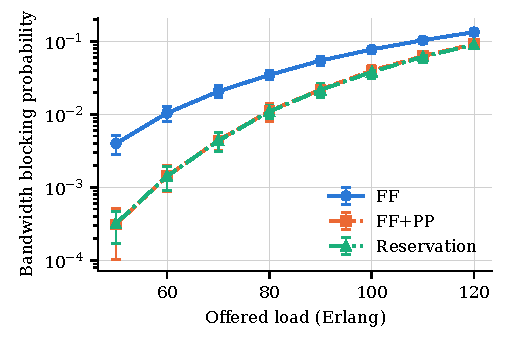
\includegraphics[width=\columnwidth]{fig_bbp.pdf}
\caption{Bandwidth blocking probability versus offered load ($\phi=0.3$, 10 seeds, 95\% confidence intervals).}
\label{fig:bbp}
\end{figure}

\begin{figure}[t]
\centering
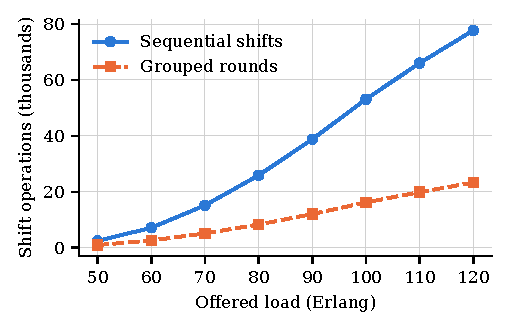
\includegraphics[width=\columnwidth]{fig_rounds.pdf}
\caption{Push-Pull shift operations per run: sequential shifts versus parallel rounds after route grouping.}
\label{fig:rounds}
\end{figure}

\subsection{Advance Reservation}
Reservation detects periodic flows with a precision of 1.00 (every reservation is used) and a recall of 0.92 at 80 Erlang, falling to 0.86 at 120 Erlang as more reservations fail for lack of spectrum. Yet its BBP stays within $-4\%$ and $+3\%$ of FF+PP at every load, inside the confidence intervals (Fig.~\ref{fig:bbp}). The reason is that with $\delta=0.2$ the block is reserved only shortly before the request arrives: when a block is free at that moment, the request would almost always have found it anyway. The paired comparison shows a small but significant benefit for periodic flows ($-13\%$ BP at 100 Erlang), with no change for random traffic.

\subsection{Zone and Hold: A Trade-Off}
Table~\ref{tab:variants} compares the variants. Hold lowers the blocking of periodic flows by 25\%, 28\%, and 36\% at 80, 100, and 120 Erlang, because their spectrum is never released between repeats. The held blocks, however, are idle until the next repeat, so random traffic is blocked 41--85\% more often and total BBP rises. At loads of 70 Erlang and below, Hold does not help periodic flows at all. Zone reduces Push-Pull shifts by 42--60\% at 80--120 Erlang because the two classes no longer interleave, but it raises total BBP by 14--45\%, since each class can use only part of the band efficiently. Combining both adds their costs. With $\phi=0$ all variants equal FF+PP, as nothing is detected; with $\phi=0.1$ Hold raises BBP from 0.039 to 0.058 at 100 Erlang.

\begin{table}[t]
\centering
\caption{Blocking and defragmentation cost of each variant ($\phi=0.3$, mean of 10 seeds)}
\label{tab:variants}
\small
\setlength{\tabcolsep}{4pt}
\begin{tabular}{@{}llrrrr@{}}
\toprule
Load & Scheme & BBP & Periodic BP & Random BP & Shifts \\
\midrule
\multirow{5}{*}{80} & FF+PP & 1.11\% & 0.74\% & 0.90\% & 25.9k \\
 & Reservation & 1.10\% & 0.69\% & 0.92\% & 26.4k \\
 & Zone & 1.61\% & 0.97\% & 1.32\% & 15.1k \\
 & Hold & 1.72\% & 0.56\% & 1.67\% & 27.3k \\
 & Zone+Hold & 2.49\% & 0.88\% & 2.33\% & 15.6k \\
\midrule
\multirow{5}{*}{100} & FF+PP & 3.99\% & 2.91\% & 3.15\% & 53.1k \\
 & Reservation & 3.81\% & 2.53\% & 3.12\% & 53.6k \\
 & Zone & 5.13\% & 3.48\% & 4.09\% & 25.8k \\
 & Hold & 5.50\% & 2.10\% & 5.21\% & 47.8k \\
 & Zone+Hold & 6.67\% & 2.65\% & 6.23\% & 21.8k \\
\midrule
\multirow{5}{*}{120} & FF+PP & 9.20\% & 7.02\% & 7.18\% & 77.7k \\
 & Reservation & 9.01\% & 6.22\% & 7.31\% & 79.7k \\
 & Zone & 10.48\% & 7.29\% & 8.38\% & 31.4k \\
 & Hold & 10.76\% & 4.52\% & 10.15\% & 62.2k \\
 & Zone+Hold & 12.39\% & 5.29\% & 11.51\% & 24.5k \\
\bottomrule
\end{tabular}
\end{table}

\subsection{Tuning the Trade-Off}
Fig.~\ref{fig:tradeoff} places each scheme by the blocking it causes to random requests and to periodic requests at 100 Erlang; points further down and to the left are better. Lengthening the reservation lead moves along a much better curve than Hold. With $\delta=1$ (about 7.5\% of the period), periodic BP falls by 29\% while total BBP does not change significantly ($-2\%$); with $\delta=2$ it falls by 44\%, at $+21\%$ random BP and no significant change in BBP ($+3\%$). Only at $\delta=5$ does the idle reserved spectrum raise BBP significantly ($+21\%$). Unrestricted Hold gives smaller protection ($-28\%$) at a much higher cost ($+65\%$ random BP, $+38\%$ BBP), because a held block stays idle for the whole gap between repeats, not just a short lead.

The Hold budget $\beta$ moves Hold between these extremes. At $\beta=0.02$, periodic BP falls significantly, by 12\% at 100 Erlang and 9\% at 120 Erlang, with no significant change in BBP. Larger budgets give more protection at more cost, and at $\beta=0.2$ Hold is almost unrestricted. The curve is not strictly monotone ($\beta=0.05$ at 100 Erlang), which reflects the noise of 10 seeds. Zone and Zone+Hold lie far from both curves: they are a way to reduce defragmentation work, not to protect periodic traffic.

\begin{figure}[t]
\centering
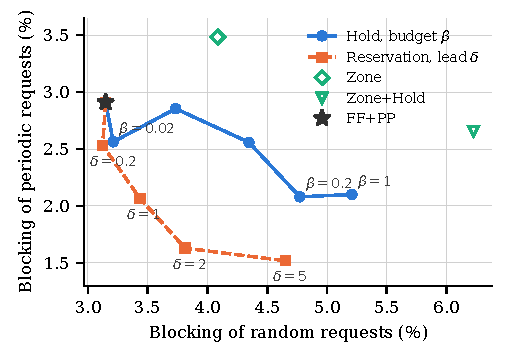
\includegraphics[width=\columnwidth]{fig_tradeoff.pdf}
\caption{Blocking of periodic versus random requests at 100 Erlang (mean of 10 seeds). Curves start at FF+PP ($\beta=0$, no lead) and vary the Hold budget $\beta$ and the reservation lead $\delta$.}
\label{fig:tradeoff}
\end{figure}

\subsection{Robustness to Timing Jitter}
Real scheduled services do not arrive exactly on time. Fig.~\ref{fig:jitter} shows Hold under arrival-time jitter. With $\varepsilon=0.1$, recall falls from 0.91 to 0.65 at $\sigma=0.05$ and to 0.24 at $\sigma=0.1$, and the protection of periodic flows disappears: their BP returns to the FF+PP level. With $\varepsilon=0.3$, recall stays above 0.9 up to $\sigma=0.05$ and is 0.82 at $\sigma=0.1$, while precision stays at 0.89--0.98 up to that point. A tolerance of about three standard deviations of the jitter is therefore needed. In practice, $\varepsilon$ can be set from the observed spread of inter-arrival times of each key.

\begin{figure}[t]
\centering
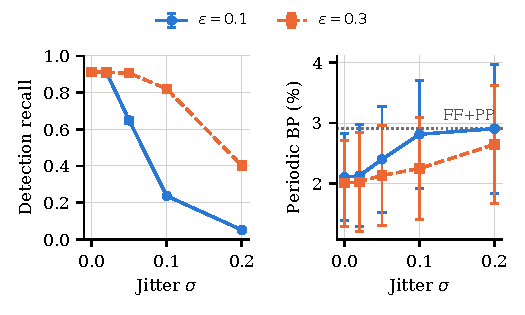
\includegraphics[width=\columnwidth]{fig_jitter.pdf}
\caption{Hold under arrival-time jitter $\sigma$ at 100 Erlang for two detection tolerances $\varepsilon$: detection recall (left) and blocking of periodic requests (right, 95\% confidence intervals).}
\label{fig:jitter}
\end{figure}

\subsection{Predictability of Demand}
Table~\ref{tab:dt} shows the decision-tree results. When 30--50\% of the load comes from periodic flows, the tree predicts high-demand windows with a precision of 0.91--0.97, but a recall of only 0.27--0.37, because only the pairs that carry periodic flows are predictable. With little or no periodic traffic, the F1-score is near zero. On the OPNET trace used in \cite{malayeri2022}, the precision of 0.54 equals the share of positive windows, i.e., chance level. Re-examining that trace showed why: its offered load is about 5{,}000 Erlang, and the generator wrote the periodic requests to a separate file, so the trace contains no recurring pattern to learn.

\begin{table}[t]
\centering
\caption{Decision-tree prediction of high-demand windows (mean of 10 seeds for synthetic traffic)}
\label{tab:dt}
\small
\begin{tabular}{@{}lrrr@{}}
\toprule
Traffic & Precision & Recall & F1 \\
\midrule
Synthetic, $\phi=0$ & 0.43 & 0.00 & 0.01 \\
Synthetic, $\phi=0.1$ & 0.52 & 0.02 & 0.03 \\
Synthetic, $\phi=0.3$ & 0.91 & 0.27 & 0.42 \\
Synthetic, $\phi=0.5$ & 0.97 & 0.37 & 0.54 \\
OPNET trace of \cite{malayeri2022} & 0.54 & 0.97 & 0.69 \\
\bottomrule
\end{tabular}
\end{table}

\subsection{Discussion}
Two lessons follow. First, the large and reliable gains come from defragmentation itself and from running it in parallel rounds. Second, recurring traffic can be detected accurately, but under the same offered load, knowing it does not free spectrum: every use of the patterns that we tested either leaves total blocking unchanged or moves blocking from one traffic class to another. This makes pattern awareness a tool for service differentiation, for example to protect scheduled video services during busy hours, rather than a way to raise total capacity. Third, of the tested mechanisms, advance reservation with a lead of about one tenth of the period gives this protection most cheaply, because it keeps spectrum idle only briefly.

\textit{Limitations.} We use one topology, a single modulation format, and strictly periodic flows with Gaussian jitter. Real traffic may contain daily patterns, flows whose period or bandwidth drifts, and flows that recur at irregular times. The simulator is open, so these cases can be added; testing them on another topology and on measured traffic is the most important next step.

% ===============================================================
\section{Conclusion}\label{sec:conclusion}
% ===============================================================
We studied whether recognizing recurring traffic patterns reduces fragmentation-induced blocking in EONs. Grouped Push-Pull defragmentation lowered blocking by 31--92\% compared with First-Fit and ran about three times faster thanks to independent-set route grouping. Periodic flows were detected with a precision of 1.00 and a recall of about 0.9, but no use of them lowered total blocking. Holding spectrum protected periodic flows (up to 36\% less blocking) and a separate zone reduced defragmentation work (up to 60\% fewer shifts), each at the expense of other traffic. Reserving spectrum about one tenth of a period ahead gave 29--44\% protection without a significant change in total blocking, and a detection tolerance of three times the timing jitter kept the recall above 0.8. Future work includes other topologies and measured traffic, priority classes for scheduled services, and reinforcement learning to decide when pattern-based actions pay off.

\section*{Acknowledgment}
\todo{Optional.}

\begin{thebibliography}{99}

\bibitem{jinno2009}
M. Jinno \textit{et al.}, ``Spectrum-efficient and scalable elastic optical path network: Architecture, benefits, and enabling technologies,'' \textit{IEEE Commun. Mag.}, vol.~47, no.~11, pp.~66--73, 2009.

\bibitem{gerstel2012}
O. Gerstel, M. Jinno, A. Lord, and S. J. B. Yoo, ``Elastic optical networking: A new dawn for the optical layer?,'' \textit{IEEE Commun. Mag.}, vol.~50, no.~2, pp.~s12--s20, 2012.

\bibitem{chatterjee2015}
B. C. Chatterjee, N. Sarma, and E. Oki, ``Routing and spectrum allocation in elastic optical networks: A tutorial,'' \textit{IEEE Commun. Surveys Tuts.}, vol.~17, no.~3, pp.~1776--1800, 2015.

\bibitem{abkenar2017}
F. S. Abkenar and A. G. Rahbar, ``Study and analysis of routing and spectrum allocation (RSA) and routing, modulation and spectrum allocation (RMSA) algorithms in elastic optical networks (EONs),'' \textit{Opt. Switch. Netw.}, vol.~23, pp.~5--39, 2017.

\bibitem{shen2015}
J. Shen, J. Chen, and Y. Sun, ``Fragmentation aware routing and spectrum assignment algorithm for elastic optical networks,'' in \textit{Proc. IEEE TENCON}, 2015.

\bibitem{athari2019}
A. Athari Beyragh, A. G. Rahbar, S.-M. Hosseini Ghazvini, and M. Nickray, ``IF-RSCA: Intelligent fragmentation-aware method for routing, spectrum and core assignment in space division multiplexing elastic optical networks (SDM-EON),'' \textit{Opt. Fiber Technol.}, vol.~50, pp.~284--301, 2019.

\bibitem{patel2011}
A. N. Patel, P. N. Ji, J. P. Jue, and T. Wang, ``Defragmentation of transparent flexible optical WDM (FWDM) networks,'' in \textit{Proc. OFC/NFOEC}, 2011.

\bibitem{wang2013}
R. Wang and B. Mukherjee, ``Provisioning in elastic optical networks with non-disruptive defragmentation,'' \textit{J. Lightw. Technol.}, vol.~31, no.~15, 2013, doi: 10.1109/JLT.2013.2268535.

\bibitem{zhang2013}
M. Zhang, W. Shi, L. Gong, W. Lu, and Z. Zhu, ``Bandwidth defragmentation in dynamic elastic optical networks with minimum traffic disruptions,'' in \textit{Proc. IEEE ICC}, 2013.

\bibitem{cugini2013}
F. Cugini \textit{et al.}, ``Push-pull defragmentation without traffic disruption in flexible grid optical networks,'' \textit{J. Lightw. Technol.}, vol.~31, no.~1, pp.~125--133, 2013.

\bibitem{shakya2013}
S. Shakya and X. Cao, ``Spectral defragmentation in elastic optical path networks using independent sets,'' in \textit{Proc. OFC/NFOEC}, 2013.

\bibitem{lu2013ar}
W. Lu and Z. Zhu, ``Dynamic service provisioning of advance reservation requests in elastic optical networks,'' \textit{J. Lightw. Technol.}, vol.~31, no.~10, pp.~1621--1627, 2013.

\bibitem{chino2016}
M. Chino, T. Miyazaki, E. Oki, S. Okamoto, and N. Yamanaka, ``Adaptive elastic spectrum allocation based on traffic fluctuation estimate in flexible OFDM-based optical networks,'' in \textit{Proc. IEEE HPSR}, 2016.

\bibitem{panayiotou2019}
T. Panayiotou, K. Manousakis, S. P. Chatzis, and G. Ellinas, ``A data-driven bandwidth allocation framework with QoS considerations for EONs,'' \textit{J. Lightw. Technol.}, vol.~37, no.~9, pp.~1853--1864, 2019.

\bibitem{salani2019}
M. Salani, C. Rottondi, and M. Tornatore, ``Routing and spectrum assignment integrating machine-learning-based QoT estimation in elastic optical networks,'' in \textit{Proc. IEEE INFOCOM}, 2019, pp.~1738--1746.

\bibitem{malayeri2022}
M. M. Malayeri, ``Optimization of fragmented spectrum in elastic optical networks using pattern recognition,'' M.Sc. thesis, Dept. Comput. Eng. IT, Univ. of Qom, Qom, Iran, 2022 (in Persian).

\bibitem{trindade2021}
S. Trindade, R. da S. Torres, Z. Zhu, and N. L. S. da Fonseca, ``Cognitive control-loop for elastic optical networks with space-division multiplexing,'' \textit{Sensors}, vol.~21, no.~23, art.~7821, 2021.

\bibitem{etezadi2022}
E. Etezadi, C. Natalino, R. Diaz, A. Lindgren, S. Melin, L. Wosinska, P. Monti, and M. Furdek, ``DeepDefrag: A deep reinforcement learning framework for spectrum defragmentation,'' in \textit{Proc. IEEE GLOBECOM}, 2022, pp.~3694--3699.

\bibitem{etezadi2023}
E. Etezadi, C. Natalino, R. Diaz, A. Lindgren, S. Melin, L. Wosinska, P. Monti, and M. Furdek, ``Deep reinforcement learning for proactive spectrum defragmentation in elastic optical networks,'' \textit{J. Opt. Commun. Netw.}, vol.~15, no.~10, pp.~E86--E96, 2023.

\bibitem{davalos2023}
E. D\'avalos, J.-L. Enciso, N. Silva, J. Pinto-R\'ios, and A. Leiva, ``Triggering strategy for defragmentation process in elastic optical networks using machine learning techniques,'' \textit{ICT Express}, vol.~9, no.~5, pp.~890--895, 2023.

\end{thebibliography}\end{document}
